\section{Related Work}

\subsection{Neural Human Avatars}
In recent years, neural radiance fields (NeRF) \cite{mildenhall2020nerf} have shown great abilities in photorealistic rendering. 
And many methods have successfully combined NeRF with human parametric models for human body reconstruction \cite{neuralbody, humannerf} and animatable human body modeling \cite{ARAH, neuman, slrf, ani-nerf, animatablenerf, peng2022animatable, selfrecon, monohuman} with sparse videos. 
For dynamic body motion modeling, people usually leverage linear blend skinning (LBS) \cite{pose_deformation} to drive the body to different poses and use neural displacement fields to model the non-rigid deformations.
Among these works, the deformation fields only model single-direction displacement, either forward deformation (canonical to observation) \cite{ARAH, tava} or backward deformation (observation to canonical) \cite{animatablenerf, ani-nerf, peng2022animatable}.
Different from them, our method proposes an invertible deformation field to solve the correspondence between canonical and observation space bidirectionally, which helps to better solve the inverse skinning problem, and leads to better geometry reconstruction.
Recent work MonoHuman \cite{monohuman} also models bidirectional deformations, but unlike the compact single invertible network in our approach, they use two non-invertible neural networks to model the deformations separately.
Additionally, these methods model body appearance using view-dependent color without decomposing it into lighting and reflectance.
In contrast, our method enables relighting by reconstructing the environment lighting and the surface material.

\subsection{Human Relighting}

Some methods have been proposed to enable relighting of human images \cite{sun2019single, wang2020single, zhou2019deep, kanamori2019relighting, pandey2021total, ji2022geometry}. However, these image-based methods do not support changing the viewpoints and human poses. 
To further enable novel view relighting, 3D reconstruction techniques have been leveraged to model the human geometry \cite{guo2019relightables}. 
For video-based human relighting, Relighting4D \cite{Relighting4D} enables free-viewpoint relighting from only human videos under unknown illuminations by using a set of neural fields of normal, occlusion, diffuse, and specular maps. 
But it is hard to relight the human with novel poses as it involves per-frame latent features which are not generalizable for novel poses. 
RANA \cite{rana} proposed a generalizable relightable articulated neural avatars creation method based on SMPL+D \cite{alldieck2018video} model with albedo, normal map refinement techniques. 
But their method did not model specular reflection and cast shadows.
In this paper, we present the first method that can reconstruct relightable and animatable human avatars from videos under unknown illuminations, while providing physically correct shadows.

\subsection{Invertible Neural Network}

Invertible Neural Networks (INNs) \cite{nice, real-nvp, i-resnet, neural-ode, glow} are are capable of performing invertible transformations between the input and output space.
They are widely used in generative models like Normalizing Flows \cite{normalizingflow} for density estimation.
Moreover, the ability of INNs to maintain cycle consistency between two spaces makes them suitable for modeling the deformation field of 3D objects. 
As a result, INNs have been used for 3D shape completion \cite{occflow, shapeflow, neural-part, cadex}, geometry processing \cite{yang2021geometry}, dynamic scenes reconstruction \cite{ndr}, and building animatable avatars with 3D scans \cite{ins}.
However, for video-based dynamic body deformation modeling, existing works only use non-invertible single-directional deformation.
In this work, we leverage the invertibility of the INNs to model the dynamic body motions and reconstruct high-quality dynamic body geometry.

\begin{figure*}[t]
\begin{center}
   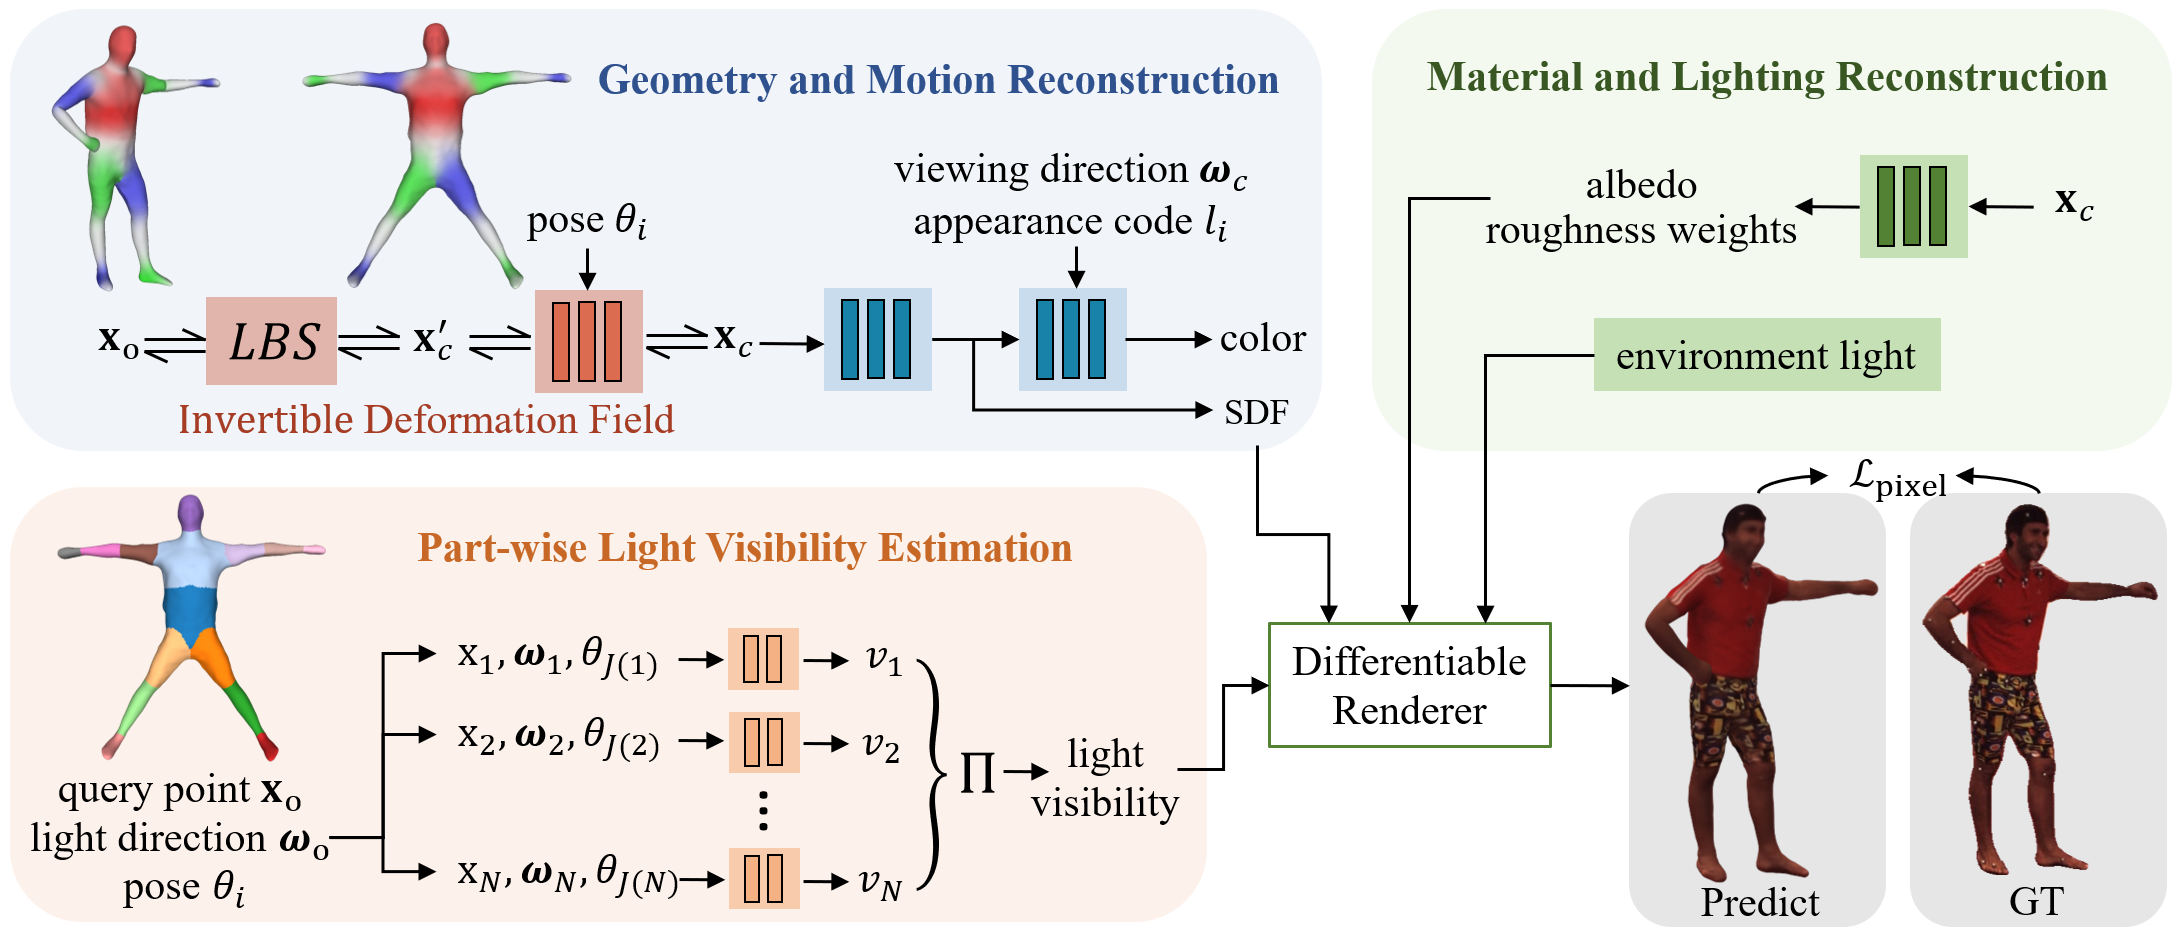
\includegraphics[width=0.95\linewidth]{./fig/pipeline.png}
\end{center}
\caption{The pipeline of our method. The invertible deformation field in \textit{Geometry and Motion Reconstruction} contributes to reconstruct more accurate dynamic body geometry (Sec.\ref{sec:geo_rec}). Then the networks in \textit{Part-wise Light Visibility Estimation} are trained to estimate pose-aware light visibility in an effective manner (Sec.\ref{sec:vis_est}). With these two parts fixed, the networks and lighting coefficients in \textit{Material and Light Estimation} are trained and optimized by the photometric losses (Sec.\ref{sec:mat_est}).}
\label{fig:pipeline}
\end{figure*}
